\newpage

\section{Trải nghiệm người dùng \& Luồng dữ liệu}

\subsection{Trải nghiệm người dùng - Quy trình hệ thống}

\subsubsection{0. Giai đoạn Matchmaking \& Cinematic}

\textbf{Mô tả:}

\begin{itemize}[topsep=0pt, itemsep=2pt, leftmargin=1.2cm]
    \item \textbf{Hàng đợi Matchmaking:} Người chơi chọn thành phố (Sài Gòn, Đà Nẵng, Hà Nội) qua màn hình \texttt{mapSelection.ts}, sau đó vào hàng đợi tìm trận. Hệ thống ghép tối đa 4 người thật; nếu sau 30s chưa đủ, bot sẽ được thêm vào cho đủ 4 người (\texttt{fillRoomWithBots} trong \texttt{server/bot.ts}).

    \item \textbf{Cinematic (Boarding Gate):} Sau khi ghép trận thành công, phòng chuyển sang phase \texttt{"cinematic"}. Màn hình boarding gate hiển thị video máy bay cất cánh, đếm ngược 7 giây, sau đó bắt đầu gameplay.

    \item \textbf{Chơi ngay (tạo phòng riêng):} Người chơi có thể tạo phòng riêng (\texttt{room:create}) để vào game ngay mà không chờ matchmaking. Bot tự động điền vào các ghế trống nhờ \texttt{fillRoomWithBots}.
\end{itemize}

\subsubsection{A. Giai đoạn Drafting (Daily Drafting Phase)}

\textbf{Mô tả:}

\begin{itemize}[topsep=0pt, itemsep=2pt, leftmargin=1.2cm]

    \item \textbf{Cơ chế phát thẻ:} Mỗi ngày, hệ thống chia 7 thẻ cho mỗi người chơi (\texttt{DRAFT\_STARTING\_POOL\_SIZE} = 7). Thực hiện 5 lượt chọn-giữ-chuyển (\texttt{HAND\_SIZE} = 5): mỗi lượt người chơi chọn giữ 1 thẻ và chuyển các thẻ còn lại theo chiều kim đồng hồ. Bot tự động pick thẻ VP cao nhất (greedy strategy) qua \texttt{server/bot.ts}. Deck được tạo cân bằng giữa 4 nhóm nhờ \texttt{createBalancedRandomDeck} trong \texttt{src/game/draft.ts}.
    
    \item \textbf{Cơ chế Vay nợ (Debt Mechanism):} Khi thiếu Xu, người chơi vẫn có thể lấy thẻ nhưng hệ thống sẽ gán ``Token Nợ''. Token này dùng để khấu trừ điểm ở bước tính toán cuối cùng.
    
    \item \textbf{Cơ chế Kiệt sức (Exhaustion):} Nếu sử dụng thẻ khi cạn Thể lực, hệ thống tự động khóa (Lock) một ô thời gian ngẫu nhiên của ngày kế tiếp, vô hiệu hóa thao tác tại ô đó.
    
    \item \textbf{Quy đổi tài nguyên (Discard):} Người chơi có quyền hủy thẻ để lấy lại một lượng Xu/Thể lực nhất định. Ô trống sau khi hủy thẻ được tính là ``Thời gian nghỉ'', giúp ngắt các ràng buộc về phạt khoảng cách.
    
\end{itemize}


\subsubsection{B. Giai đoạn Lên lịch trình}

\textbf{Mô tả:}

\begin{itemize}[topsep=0pt, itemsep=2pt, leftmargin=1.2cm]

    \item \textbf{Phân bổ Grid:} Người dùng thực hiện chọn và kéo thả thẻ bài vào các slot Sáng - Trưa - Chiều - Tối - Khuya trên Grid 5×5 (5 ngày × 5 khung giờ).
    
    \item \textbf{Chốt ngày:} Sau khi xác nhận lịch trình trong ngày, các thẻ chưa sử dụng trong kho sẽ bị hủy để giải phóng bộ nhớ cho ngày làm việc tiếp theo.
    
\end{itemize}

\subsubsection{C. Giai đoạn Simulation \& Scoring}

\textbf{Mô tả:} Sau mỗi ngày (khi người chơi xác nhận planning), hệ thống khóa Grid của ngày đó và thực hiện chuỗi thuật toán tính điểm tự động gồm 5 bước. Vòng lặp này lặp lại cho tất cả 5 ngày. Sau ngày thứ 5, hệ thống chuyển sang phase \texttt{"result"} hiển thị các bước replay (từng sự kiện, combo, khoảng cách) rồi mới đến màn hình Game Over với tổng kết điểm VP cuối cùng.
    
\begin{itemize}[topsep=0pt, itemsep=2pt, leftmargin=1.2cm]

    \item \textbf{Bước 1 (Check Nợ):} Kiểm tra số lượng Token Nợ và thực hiện trừ điểm tương ứng.
    
    \item \textbf{Bước 2 (Random Events):} Chạy xác suất 15\% kích hoạt sự kiện dựa trên tag của thẻ (thời tiết, giao diện, sức khỏe). Kết quả được tính bằng hàm hash có seed (không dùng Math.random), đảm bảo tái tạo được giống hệt khi cùng input. Sự kiện tác động $\pm$10 VP hoặc -8 Thể lực.
    
    \item \textbf{Bước 3 (Check Combo):} Duyệt Grid theo từng ngày (cột) để tìm các Tag khớp với bộ quy tắc Combo (\texttt{src/game/combos.ts}): theme (FOOD/CULTURE/ACTION), secondary (INDOOR/OUTDOOR), tag-pair, slot/rhythm, risk/reward. Điểm thưởng được cộng tự động.
    
    \item \textbf{Bước 4 (Check Distance):} Tính toán khoảng cách giữa các thẻ liền kề. Nếu vượt quá 20km/di chuyển, hệ thống áp dụng điểm phạt. Nếu có ô trống ở giữa, thuật toán sẽ bỏ qua bước kiểm tra này.
    
    \item \textbf{Bước 5 (Final VP):} Tổng hợp điểm gốc, Bonus Combo và các khoản Penalty để xuất kết quả cuối cùng cho ngày đó.
    
\end{itemize}

\subsubsection{D. Chuyển đổi Phase (Chưa triển khai)}
    
Tính năng Campaign Progression (chơi nối tiếp nhiều phase) chưa được triển khai. Tuy nhiên, dữ liệu thẻ đã có sẵn cho 3 thành phố: \textbf{Sài Gòn (Phase 1)}, \textbf{Đà Nẵng (Phase 2)} trong \texttt{cards.phase2.ts}, và \textbf{Hà Nội (Phase 3)} trong \texttt{cards.phase3.ts}. Người chơi có thể chọn thành phố khi bắt đầu game qua \texttt{mapSelection.ts}. Kế hoạch mở rộng bản đồ gồm các nhánh Đà Lạt, Nha Trang, Huế được giữ lại cho các phiên bản tương lai.

\subsubsection{E. Xuất dữ liệu}

\textbf{Mô tả logic:} Hệ thống chuyển đổi toàn bộ Grid thành định dạng Timeline báo cáo sau khi kết thúc 5 ngày.

\textbf{Nội dung Export:} Danh sách địa điểm cụ thể, tổng quãng đường di chuyển, dự toán chi phí và chứng chỉ du lịch (\texttt{src/export/certificate.ts}). File này giúp người dùng có thể sử dụng như một lịch trình du lịch thực tế.
    
\newpage

\subsection{Luồng dữ liệu}

\subsubsection{Thành phần tham gia}

\begin{itemize}[topsep=0pt, itemsep=2.5pt, leftmargin=1.5cm]
    \item Người dùng - Tạo ra các input chính như đăng nhập, chọn thẻ, kéo thả thẻ vào grid, xác nhận vay tài nguyên, chọn tuyến hành trình và chạy mô phỏng.

    \item Lớp giao diện UI - Chịu trách nhiệm hiển thị:
    \begin{itemize}[label=\ding{111}, leftmargin=1.5cm]
        \item Màn hình đăng nhập và hồ sơ
        \item Bộ thẻ hiện có, bàn cờ lịch trình 5x5, thanh tài nguyên
        \item Popup xác nhận và cảnh báo
        \item Kết quả mô phỏng, điểm VP và tiến trình phase
    \end{itemize}

    \item Frontend Logic - Frontend tiếp nhận thao tác từ UI, chuẩn hóa dữ liệu đầu vào, kiểm tra hợp lệ cơ bản và gửi request sang backend. Đồng thời frontend nhận phản hồi để cập nhật giao diện ngay lập tức.

    \item Backend / Game Engine - Xử lý logic gameplay gồm:
    \begin{itemize}[label=\ding{111}, leftmargin=1.5cm]
        \item Kiểm tra tài nguyên, kiểm tra điều kiện đặt thẻ
        \item Tính combo và synergy
        \item Thanh tài nguyên
        \item Áp dụng debt token, exhaustion và penalty
        \item Mô phỏng random events, distance check và final VP
    \end{itemize}

    \item Lưu trữ:
        \begin{itemize}[label=\ding{111}, leftmargin=1.5cm]
        \item Hồ sơ người chơi: lưu trong PostgreSQL (\texttt{server/db.ts}) với bảng \texttt{users}, mật khẩu băm PBKDF2. Server vẫn chạy được ở chế độ không-DB nếu chưa cấu hình \texttt{DATABASE\_URL}.
        \item Trạng thái phòng chơi: sống trong bộ nhớ (in-memory) trên server Node.js.
        \item Lịch sử ván chơi: lưu trong PostgreSQL qua các bảng \texttt{matches} và \texttt{match\_players} (\texttt{saveMatchResult}).
        \item Cache tài nguyên PWA qua Service Worker (\texttt{sw.js}).
    \end{itemize}
\end{itemize}

\subsubsection{Tổng quan luồng dữ liệu}

\begin{figure}[H]
    \centering
    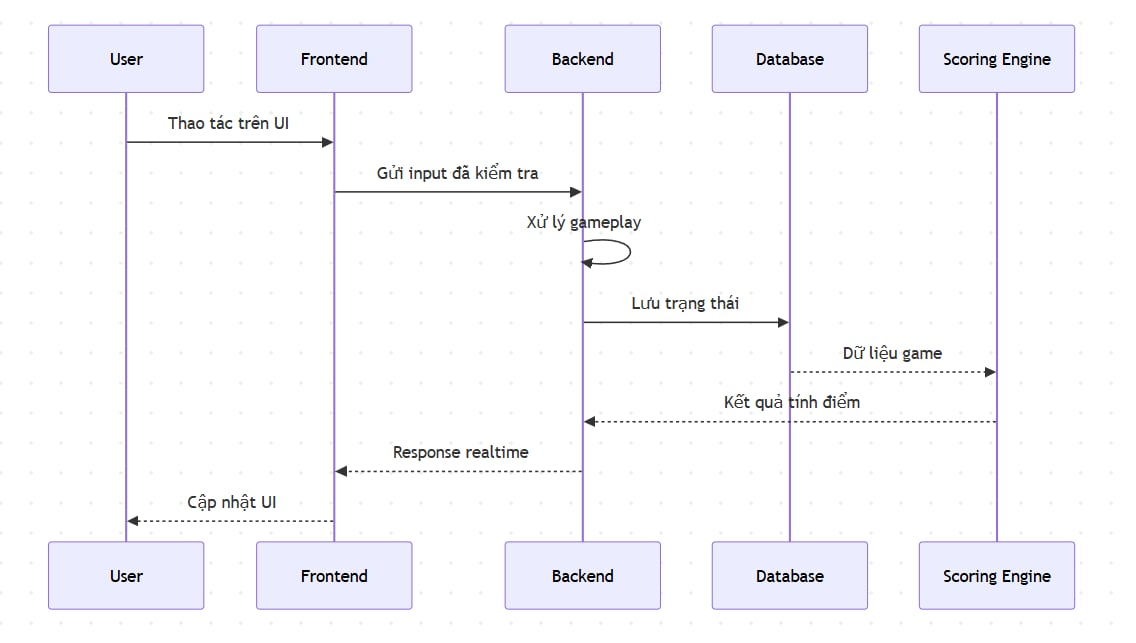
\includegraphics[width=1\textwidth]{images/part5/data-flow.jpg}
    \caption{Sơ đồ Data Flow} 
\end{figure}

\subsection{Luồng dữ liệu theo từng giai đoạn UI/UX}

\subsubsection{Giai đoạn đăng nhập và truy cập hệ thống}

Đây là điểm bắt đầu của luồng dữ liệu. Người dùng nhập email hoặc username cùng password trên màn hình đăng nhập.

\begin{itemize}[topsep=0pt, itemsep=2.5pt, leftmargin=1.5cm]
    \item \textbf{Input từ UI:}
    \begin{itemize}[topsep=0pt, itemsep=2pt]
        \item Email hoặc Username
        \item Password
    \end{itemize}

    \item \textbf{Xử lý:}
    \begin{itemize}[topsep=0pt, itemsep=2pt]
        \item Frontend kiểm tra định dạng dữ liệu
        \item Backend xác thực tài khoản
        \item Database trả về hồ sơ và tiến trình người chơi
    \end{itemize}

    \item \textbf{Output trả về UI:}
    \begin{itemize}[topsep=0pt, itemsep=2pt]
        \item Hồ sơ người chơi
        \item Lịch sử trận đấu
        \item Tiến trình tài khoản
        \item Trạng thái đăng nhập thành công hoặc lỗi xác thực
    \end{itemize}
\end{itemize}

\subsubsection{Giai đoạn Drafting}

Mỗi ngày hệ thống cấp 7 thẻ cho người chơi. Người chơi chọn giữ thẻ, chuyển phần còn lại và lặp qua các lượt draft.

\begin{itemize}[topsep=0pt, itemsep=2.5pt, leftmargin=1.5cm]
    \item \textbf{Input từ UI:}
    \begin{itemize}[topsep=0pt, itemsep=2pt]
        \item Bộ thẻ được phát
        \item Lựa chọn giữ thẻ
        \item Hành động bỏ thẻ hoặc xác nhận lượt
    \end{itemize}

    \item \textbf{Xử lý:}
    \begin{itemize}[topsep=0pt, itemsep=2pt]
        \item Frontend ghi nhận thẻ được chọn
        \item Backend cập nhật pool thẻ, trạng thái lượt và chiến thuật tạm thời
        \item Nếu thiếu Xu mà vẫn lấy thẻ, hệ thống gán Token Nợ
        \item Nếu thiếu Thể Lực mà vẫn dùng thẻ, hệ thống kích hoạt cơ chế Kiệt Sức và khóa ô tương lai
    \end{itemize}

    \item \textbf{Output trả về UI:}
    \begin{itemize}[topsep=0pt, itemsep=2pt]
        \item Bộ thẻ cuối cùng sau draft
        \item Trạng thái tài nguyên hiện tại
        \item Token Nợ nếu phát sinh
        \item Cảnh báo rủi ro nếu chọn vượt tài nguyên
    \end{itemize}
\end{itemize}

\subsubsection{Giai đoạn xây dựng lịch trình trên Grid 5x5}

Người dùng kéo thả thẻ vào grid gồm 5 hàng thời gian và 5 cột ngày để tạo lịch trình.

\begin{itemize}[topsep=0pt, itemsep=2.5pt, leftmargin=1.5cm]
    \item \textbf{Input từ UI:}
    \begin{itemize}[topsep=0pt, itemsep=2pt]
        \item Thẻ được chọn
        \item Vị trí thả thẻ trên grid
        \item Hành động đổi chỗ, hủy thẻ hoặc chốt ngày
    \end{itemize}

    \item \textbf{Xử lý:}
    \begin{itemize}[topsep=0pt, itemsep=2pt]
        \item Frontend gửi card id, vị trí ô và trạng thái thao tác
        \item Backend kiểm tra:
        \begin{itemize}[topsep=0pt, itemsep=1.5pt]
            \item Ô có hợp lệ không
            \item Tài nguyên có đủ không
            \item Thẻ có gây xung đột hoặc vi phạm luật không
            \item Combo nào được kích hoạt
            \item Khoảng cách di chuyển có vượt ngưỡng không
        \end{itemize}
        \item Kết quả được lưu lại theo trạng thái board hiện tại
    \end{itemize}

    \item \textbf{Output trả về UI:}
    \begin{itemize}[topsep=0pt, itemsep=2pt]
        \item Grid đã cập nhật
        \item Combo đang kích hoạt
        \item Preview điểm VP tạm thời
        \item Tài nguyên còn lại
        \item Cảnh báo lỗi nếu đặt sai vị trí
    \end{itemize}
\end{itemize}

\subsubsection{Giai đoạn quản lý tài nguyên}

Song song với việc xếp thẻ, hệ thống luôn theo dõi Xu Vàng, Thể Lực và các trạng thái phát sinh.

\begin{itemize}[topsep=0pt, itemsep=2.5pt, leftmargin=1.5cm]
    \item \textbf{Input từ UI:}
    \begin{itemize}[topsep=0pt, itemsep=2pt]
        \item Hành động mua thẻ
        \item Quyết định vay tài nguyên
        \item Hành động hủy thẻ để đổi lại tài nguyên
    \end{itemize}

    \item \textbf{Xử lý:}
    \begin{itemize}[topsep=0pt, itemsep=2pt]
        \item Backend kiểm tra số dư tài nguyên
        \item Nếu vay Xu, hệ thống tạo Token Nợ
        \item Nếu dùng quá Thể Lực, hệ thống sinh trạng thái khóa ô
        \item Nếu hủy thẻ, hệ thống hoàn lại tài nguyên theo luật
        \item Thẻ Utility có hiệu ứng đặc biệt (\texttt{onPlayEffect}): hồi Xu/Thể lực (RECOVER\_XU, RECOVER\_LA), miễn phạt khoảng cách (IGNORE\_DISTANCE\_NEXT), giảm giá (DISCOUNT\_XU\_NEXT), nhân đôi VP (DOUBLE\_VP\_NEXT).
    \end{itemize}

    \item \textbf{Output trả về UI:}
    \begin{itemize}[topsep=0pt, itemsep=2pt]
        \item Chỉ số tài nguyên mới
        \item Trạng thái penalty
        \item Popup xác nhận hoặc cảnh báo
        \item Gợi ý hậu quả cho lượt tiếp theo
    \end{itemize}
\end{itemize}

\subsubsection{Giai đoạn Simulation \& Scoring}

Sau khi người dùng hoàn tất lịch trình, hệ thống khóa grid và chạy chuỗi mô phỏng chấm điểm.

\begin{itemize}[topsep=0pt, itemsep=2.5pt, leftmargin=1.5cm]
    \item \textbf{Input từ UI / hệ thống:}
    \begin{itemize}[topsep=0pt, itemsep=2pt]
        \item Grid lịch trình cuối cùng
        \item Dữ liệu tag thẻ
        \item Tọa độ địa điểm
        \item Trạng thái Token Nợ, Exhaustion và các penalty khác
    \end{itemize}

    \item \textbf{Xử lý trong backend:}
    \begin{enumerate}[topsep=0pt, itemsep=2pt]
        \item Kiểm tra Token Nợ và trừ điểm tương ứng.
        \item Kích hoạt random events theo xác suất 15\% dựa trên tag, dùng hàm hash có seed để đảm bảo tái tạo được.
        \item Duyệt combo theo hàng và cột để cộng thưởng.
        \item Kiểm tra khoảng cách giữa các điểm liền kề, áp dụng phạt nếu vượt 20km.
        \item Tổng hợp điểm gốc, bonus và penalty để ra Final VP.
    \end{enumerate}

    \item \textbf{Output trả về UI:}
    \begin{itemize}[topsep=0pt, itemsep=2pt]
        \item Tổng điểm VP
        \item Danh sách combo đạt được
        \item Các sự kiện ngẫu nhiên đã kích hoạt
        \item Thống kê quãng đường, chi phí và hiệu quả hành trình
    \end{itemize}
\end{itemize}

% \subsubsection{Giai đoạn chuyển phase và mở rộng bản đồ}

% Sau khi kết thúc một phase, người chơi chọn hướng di chuyển để mở khóa phase tiếp theo.

% \begin{itemize}[topsep=0pt, itemsep=2.5pt, leftmargin=1.5cm]
%     \item \textbf{Input từ UI:}
%     \begin{itemize}[topsep=0pt, itemsep=2pt]
%         \item Lựa chọn tuyến đường
%         \item Hình thức di chuyển
%         \item Quyết định trả bằng Xu hoặc Thể Lực
%     \end{itemize}

%     \item \textbf{Xử lý:}
%     \begin{itemize}[topsep=0pt, itemsep=2pt]
%         \item Backend kiểm tra điều kiện mở khóa
%         \item Cập nhật branch campaign
%         \item Mở bộ thẻ và khu vực mới tương ứng
%     \end{itemize}

%     \item \textbf{Output trả về UI:}
%     \begin{itemize}[topsep=0pt, itemsep=2pt]
%         \item Bản đồ phase tiếp theo
%         \item Tuyến hành trình mới
%         \item Thẻ mới được mở khóa
%         \item Định hướng chiến thuật mới
%     \end{itemize}
% \end{itemize}

\subsubsection{Giai đoạn xuất dữ liệu}

Sau mô phỏng, hệ thống có thể chuyển toàn bộ grid thành định dạng timeline phục vụ báo cáo hoặc tái sử dụng như lịch trình du lịch thực tế.

\begin{itemize}[topsep=0pt, itemsep=2.5pt, leftmargin=1.5cm]
    \item \textbf{Input:}
    \begin{itemize}[topsep=0pt, itemsep=2pt]
        \item Grid cuối cùng
        \item Kết quả chấm điểm
        \item Thông tin khoảng cách và chi phí
    \end{itemize}

    \item \textbf{Output:}
    \begin{itemize}[topsep=0pt, itemsep=2pt]
        \item Timeline hành trình
        \item Danh sách địa điểm
        \item Tổng quãng đường
        \item Dự toán chi phí
    \end{itemize}
\end{itemize}

